%%%%%%%%%%%%%%%%%%%%%%%%%%%%%%%%%%%%%%%%%%%%%%%%%%%%%%%%%%%%%%%%%%%%%%%%%%%%%%%%%%%
%%Anna University sample latex thesis format for UG thesis
%--------------------------------
%%This is the main file that includes the front matter and other chapter links. 
%%Chapters are placed within the folder named 1, 2,...  
%%To compile, run the command `pdflatex authesis.tex' in the terminal. 
%%Some packages may not be needed. Comment the ones, that are not needed. 
%%Images can be saved in the format of *.png. 
%%------------------------------------------------------
%% Authors:
%%Originally used by Dr. Mary Anita Rajam and then modified by Dr. Bama Srinivasan according to the latest Anna University regulations. %%Please report changes to bama@annauniv.edu, chorse@gmail.com %%
%%Acknowledgement: Thanks to Dr.Ranjani Parthasarathi, who relentlessly and patiently guided Bama Srinivasan.
%---------------------------------------------------------
%% Modification added:
%%new file apalikem is added, which gives a neat reference list with 1, 2...
%%aureportm has appendix starting with Arabic numbers
%% Disclaimer: Check with the latest Anna University regulations before working with this format.
%% Changes as on July 2016 
%% 1. Changed the appendix back to alpha mode in aureport.cls
%% 2. Table of contents - reduced the top margin and spacing
%% 3. Added the counter depth for sections to 4 in aureport.cls
%% 4. Deleted chapter number, title and page number in TOC
%% 5. Reduced the top space in chapter titles from 6.5 cms to 5.5 cms in aureport.cls
%% 6. Changes in references use the package natbib and style unsrt. Include a .bib file for the bibliography
%$$$$$$$$$$$$$$$$$$$$$$$$$$$$$$$$$$$$$$$$$$$$$$$$$$$$$$$$$$$$$$$$$$$$$$$$$$$$$$$$$$$$$$$$$$

\documentclass[13 pt,a4paper]{aureportm}
\usepackage{mathptm}\usepackage{etex}
\reserveinserts{28}
\renewcommand{\normalsize}{\fontsize{13 pt}{14.6 pt}\selectfont}
%\usepackage{aunatbib}
%\usepackage{apalikem}
\usepackage{natbib}
\usepackage{bussproofs} % for deduction rules 
\usepackage{auphd}
\usepackage{array}
\usepackage{tabularx}
\usepackage[none]{hyphenat}
\usepackage[chapter]{algorithm}
\usepackage{algpseudocode}
\usepackage{multirow}
\usepackage{multicol}
\usepackage{float}
\usepackage{booktabs}
\usepackage{amsmath}
\usepackage{amssymb}
\usepackage{amsthm}
\usepackage{latexsym}
\usepackage{verbatim}
\usepackage{ifthen}
\usepackage{graphicx}
\usepackage{hyperref}
\usepackage{epsfig}
\usepackage{pslatex}
\usepackage{setspace}
\usepackage{titlesec}
\usepackage[subfigure]{tocloft}
\usepackage{subfigure}
\usepackage{longtable}
\usepackage{enumerate}
\usepackage{lscape}

\usepackage[format=hang,labelfont=bf,textfont=bf]{caption}
\PassOptionsToPackage{linktocpage}{hyperref}
\tocloftpagestyle{myheadings}
\newcommand{\PreserveBackslash}[1]{\let\temp=\\#1\let\\=\temp}
\let\PBS=\PreserveBackslash

\usepackage{colortbl}
\usepackage{newlfont}


\newboolean{psoutput}
\setboolean{psoutput}{true}
%\usepackage{pst-all}
\newcommand{\defname}[1]{\emph{#1}.}

\newtheorem{fact}{Fact}[chapter]

\floatstyle{ruled}
\newfloat{algorithm}{htp}{loa}
\floatname{algorithm}{Algorithm}


\titleformat{\section}[hang]{\bfseries}{\makebox[20mm][l]{\thesection}}{0pt}{}{}
\titleformat{\subsection}[hang]{\bfseries}{\makebox[20mm][l]{\thesubsection}}{0pt}{}{}



 \newcounter {definition}[chapter]
\renewcommand \thedefinition {\arabic{chapter}.\arabic{definition}}
\newenvironment{definition}
{ \refstepcounter{definition}
   {\noindent \bf Definition \arabic{chapter}.\arabic{definition}.}}
 {}
 \def\enddefinition{$\Box$}

 \newcounter {example}[chapter]
 \renewcommand \theexample
 {\arabic{chapter}.\arabic{example}}
 \newenvironment{example}
 { \refstepcounter{example}
   {\noindent \bf Example \arabic{chapter}.\arabic{example}.}}
 {}
 \def\endexample{$\Box$}

 \newcounter {proposition}[chapter]
 \renewcommand \theproposition {\arabic{chapter}.\arabic{proposition}}
 \newenvironment{proposition}
 {\refstepcounter{proposition}
   {\noindent \bf Proposition \arabic{chapter}.\arabic{proposition}. }}
 {}
 \def\endproposition{$\Box$}

\pagenumbering{roman}
\setcounter{page}{3}
%\setcounter{secnumdepth}{3}
\renewcommand{\baselinestretch}{1.5}
\newcommand{\row}{i}
\newcommand {\combined} {{C}}
\newcommand {\mtis} {}

\newboolean{showalter}
\setboolean{showalter}{true}
\newcommand{\alter}[1]{\ifthenelse{\boolean{showalter}}{ \{ #1 \} }{}}
\providecommand{\tabularnewline}{\\}
\newcommand{\bigsize}{\fontsize{15pt}{20pt}\selectfont}

\author{Author of the thesis}


\renewcommand{\cfttoctitlefont}{\bfseries\Large}
\renewcommand{\cftlottitlefont}{\bfseries\Large}
\renewcommand{\cftloftitlefont}{\bfseries\Large}


%\cftsetindents{chapter}{0mm}{10mm}
%\cftsetindents{section}{10mm}{10mm}
%\cftsetindents{subsection}{20mm}{10mm}
%\setlength{\cftbeforechapskip}{1.2\baselineskip}
%\setlength{\cftbeforesecskip}{.8\baselineskip}
%\setlength{\cftbeforesubsecskip}{.8\baselineskip}
%\setlength{\cftbeforefigskip}{.8\baselineskip}
%\setlength{\cftbeforetabskip}{.8\baselineskip}
%
\makeatletter
\renewcommand{\@dotsep}{10}
\makeatother
\renewcommand{\cftdot}{ }
\cftsetrmarg{1.2in} % changed by bama - earlier it was 1.5 inch. right margin is decreased to 1 inch.

\titleformat{\section}[hang]{\bfseries}{\makebox[20mm][l]{\thesection}}{0pt}{}{}
\titleformat{\subsection}[hang]{\bfseries}{{\thesubsection}}{0pt}{}{}
\titleformat{\subsubsection}[hang]{\normalsize\bfseries}{\makebox[20mm][l]{\thesubsubsection}}{0pt}{}{}
\titleformat{\paragraph}[hang]{\normalsize\bfseries}{\makebox[20mm][l]{\theparagraph}}{0pt}{}{}
\titleformat{\subparagraph}[hang]{\normalsize\bfseries}{\makebox[20mm][l]{\thesubparagraph}}{0pt}{}{}

\begin{document}

\pagenumbering{roman}


\thispagestyle{empty}
\begin{center}
  \LARGE
  \textbf{\uppercase{The Milkman}} \\
  \vspace{0.6\baselineskip}
  \bigsize{\textbf{A PROJECT REPORT}}\\
 \vspace{0.4\baselineskip}

  \normalsize{\textit{\textbf{Submitted by}}}\\
  \vspace{0.5\baselineskip}
  {
  \Large \textbf{SAIVARSHINI RAVICHANDRAN 2016115083}}\\
  %\normalsize{\tVextbf{(Roll number)}}\\
  \Large{\textbf{ARUN KUMAR G 2016115009}}\\
  \Large{\textbf{AJITHA GOMATHY A 2016115005}} \\
   \vspace{0.6\baselineskip}
  %\normalsize{\textit{A report for the phase-I of the project}}\\
  \vspace{-0.1\baselineskip}
  \normalsize{\textit{submitted to the Faculty of}} \\
  \vspace{0.5\baselineskip}
  \normalsize{\textbf{INFORMATION AND COMMUNICATION ENGINEERING}} \\  
  \vspace{1\baselineskip}
  \normalsize{\textit{in partial fulfillment  for the award of the degree}}\\
  \normalsize{\textit{\textbf{of}}}\\
\vspace{.2\baselineskip}
  \bigsize{{\textbf{BACHELOR OF TECHNOLOGY}}}\\
  \normalsize{\textit{\textbf{in}}}\\
  \bigsize{{\textbf{INFORMATION TECHNOLOGY}}}\\
\end{center}
  \begin{center}
   %
\includegraphics[width=26mm,height=25mm]{auemblem.pdf}   \\
   
\includegraphics[scale=0.7]{auemblem.pdf} \\
  \normalsize{ \textbf{DEPARTMENT OF INFORMATION SCIENCE AND TECHNOLOGY }}\\
  \normalsize{\textbf{COLLEGE OF ENGINEERING, GUINDY}}\\
  \normalsize{\textbf{ANNA UNIVERSITY}}\\
  \normalsize{\textbf{CHENNAI  600 025}}\\
  \vspace{0.5\baselineskip}
  \normalsize{\textbf{MONTH YEAR }}
 \end{center}
\pagebreak


\iffalse
\chapter*{ANNA UNIVERSITY\\
CHENNAI - 600 025\\
%\vspace{\baselineskip}
BONA FIDE CERTIFICATE}
\newlength{\aulength}
\settowidth{\aulength}{Anna University
  Chennai}
\newlength{\datewidth}
\settowidth{\datewidth}{Chennai 600 025}

\begin{spacing}{1.5}
  \begin{sloppypar}
  \fontsize{13}{14.5}\selectfont Certified that this project report titled TITLE OF THE PROJECT TITLE OF THE PROJECT TITLE OF THE PROJECT TITLE OF THE PROJECT TITLE OF THE PROJECT is the bona fide work of NAME OF THE CANDIDATE(S) who carried out project work under my supervision. Certified further that to the best of my knowledge and belief, the work reported herein does not form part of any other thesis or dissertation on the basis of which a degree or an award was conferred on an earlier occasion on this or any other candidate.
  \end{sloppypar}
\end{spacing}
\vspace{-0.3 cm}
\begin{flushleft}
 \parbox[t]{\datewidth}{\small{\textbf{PLACE: }}\\
 \small{\textbf{DATE: }}}
 \hfill
 \parbox[t]{6 cm}{\small{\textbf{$<$NAME OF GUIDE$>$}} \\
 \small{\textbf{$<$DESIGNATION$>$}}\\
 \small{\textbf{PROJECT GUIDE}}\\
 \small{\textbf{DEPARTMENT OF IST, CEG}}\\
 \small{\textbf{ANNA UNIVERSITY}}   \\
 \small{\textbf{CHENNAI  600025}}
 }
\end{flushleft}
%\vspace{0.5 cm}
\begin{center}
 \small{\textbf{COUNTERSIGNED}}\\ 
  \vspace{1.5 cm}
  \textbf{\small{Dr. SASWATI MUKHERJEE}}\\ 
  \small{\textbf{HEAD OF THE DEPARTMENT}}\\
 \small{\textbf{DEPARTMENT OF INFORMATION SCIENCE AND TECHNOLOGY}}\\
 \small{\textbf{COLLEGE OF ENGINEERING, GUINDY}}\\
 \small{\textbf{ANNA UNIVERSITY}}   \\
 \small{\textbf{CHENNAI  600025}}
 
\end{center}

\fi

%\addtocontents{toc}{\protect\flushleft \protect\bfseries
%CHAPTER NO. \hfill TITLE \hfill PAGE NO.\endgraf}

%\addtocontents{toc}{\protect\raggedleft Page\\}

 %\addtocontents{lof}{\protect\flushleft
%\protect\bfseries FIGURE NO. \hfill
% TITLE \hfill  PAGE NO.\endgraf}%
%\addtocontents{lot}{\protect\flushleft \protect\bfseries TABLE NO. \hfill
%  TITLE \hfill  PAGE NO.\endgraf}%


\chapter*{\uppercase{ABSTRACT}}
\addcontentsline{toc}{section}{\bfseries \uppercase{Abstract}}
India is one of the highest milk producing countries. With the increase in population, consumers are growing day by day. Due to the varying milk requirements of the people, it becomes difficult for the milkmen to keep track of everyone’s varying needs. Also, with the growth in milk production, there is a lack of an efficient mechanism to collect milk from the producers, i.e., farmers. How can this be made more efficient using technology?

Our project aims to make the milk collection and distribution better by building an
application for the large-scale cooperative societies like Aavin that collect milk from
farmers, package them and sell them to consumers. Through our application, the
consumers will be able to make changes to their daily milk requirements. Also the milk
producers, i.e., farmers, will be able to benefit by selling their milk in a quick and efficient
manner.

This  application will provide interface to its customers, where they will be able to update their requirements on a regular basis. In addition to this, they will also be able to track their consumption. The farmers who produce milk can sell it to the society as and when theywant, by listing in the app which will be collected by one of the distributors. The distributors perform the processes of both collection and distribution a The administrators will be able to monitor other users and the application will have provisions to track location of the distributors on a lively basis. 
%\chapter*{\uppercase{ACKNOWLEDGEMENT}}
%\addcontentsline{toc}{section}{\bfseries \uppercase{Acknowledgement}}
Acknowledgement should be brief and should not exceed one page when typed in one and a half line spacing.

\setlength\cftparskip{0pt}
\setlength{\cftbeforetoctitleskip}{-3em} %Decrease the top margin of toc title
%\setlength{\cftaftertoctitleskip}{0 em} 
\setlength{\cftbeforelottitleskip}{-3em} % Decrease the top margin of lot
\setlength{\cftbeforeloftitleskip}{-3em} % Decrease the top margin of lof
\cftsetindents{chapter}{0 mm}{10 mm}
\cftsetindents{section}{10 mm}{10 mm}
\cftsetindents{subsection}{20 mm}{10 mm}
\cftsetindents{subsubsection}{30 mm}{15 mm}
\cftsetindents{paragraph}{40 mm}{20 mm}
\cftsetindents{subparagraph}{50 mm} {20  mm}
\cftsetindents{table}{10 mm}{10 mm}
\cftsetindents{figure}{10 mm}{10 mm}
%%%%%%%%%%%%%%%%%%%%%%%%%%%%%%%%%%%%%%%%%%%%%%%
%Changes made as on June 2016
%%%%%%%%ADD TOC with one half spacing%%%%%%%%%%%
\begin{onehalfspacing} 
\tableofcontents

\pagebreak

\iffalse
\addcontentsline{toc}{section}{\bfseries LIST OF TABLES}
\listoftables

 \clearpage \addcontentsline{toc}{section}{\bfseries
LIST OF FIGURES} \listoffigures
%\clearpage
\fi
\end{onehalfspacing}
%%%%%%%%%%%%%%%%%%%%%%%%%%%%%%%%%%%%%%%%%%%%%%
% These are old as of April 2016 -
%%%%%%%%%%%%%%%%%%%%%%%%%%%%%%%%%%%%%%%%%%%%%%%%
%\cftsetindents{chapter}{0.2in}{1.5in}
%\cftsetindents{section}{1.7in}{0.3in}
%\cftsetindents{subsection}{1.8in}{0.4in}
%\cftsetindents{table}{0.2in}{1.5in}
%\cftsetindents{figure}{0.2in}{1.5in}
%\tableofcontents



%\pagebreak

%\addcontentsline{toc}{section}{\bfseries LIST OF TABLES}
%\listoftables
% \clearpage \addcontentsline{toc}{section}{\bfseries
%LIST OF FIGURES} \listoffigures
%\clearpage
%%%%%%%%%%%%%%%%%%%%%%%%%%%%%%%%%%%%%%%%%%%%%%%%%%%%%%%%%%%
%\chapter*{LIST OF SYMBOLS AND ABBREVIATIONS}
\addcontentsline{toc}{section}{\bfseries LIST OF SYMBOLS AND ABBREVIATIONS}

\setlongtables
\begin{longtable}
  {>{\PBS\raggedright\hspace{0pt}}p{3cm}@{}%
    >{\PBS\raggedright\hspace{0pt}}p{11.5cm}@{}}

  %$A$ & Set of attributes\\ 
  %$a_t$ & Time attribute\\
  $-$, $\neg$, $\sim$  & Negation operator \\
  $+$, $\vee$, $\cup$ & Disjunction operator \\
  $X$, $\wedge$ & Conjunction operator \\
  $\rightarrow$ & Conditional operator \\
  $\leftrightarrow$ & Biconditional operator \\
  $\diamond$ & Future tense modal operator\\
  $\alpha$ & Action \\    
  \end{longtable}
%\end{tabular}

%\clearpage

%\newpage
\pagenumbering{arabic}

\ausection
% Chapter 1

\chapter{\uppercase{Introduction}} % Main chapter title
\label{intro} % For referencing
In todays era, there are many cities which are working on transforming
themselves into Smart Cities.If the city is going to be called as Smart City,
then it should have all possible advancements in the sector of smart technology.
Improving efficiency in agriculture sector if one of the difficult and most challenging
jobs. Milk, being considered to be a staple diet among Indians, there is a lack of efficient milk delivery system. Through an android application, with one click the farmers will also be able to sell their products and the consumers will able to receive their requirements at an ease. 

Our android application can help to communicate between the farmer, distributor and customer which is implemented in this project. Android application is designed in such a way that time complexity will be minimized extensively. This is achieved by exchanging only the required data with server in order to minimize the traffic and loss of data packets in the process of delivery. With the help of cutting edge technology and keeping the goal in mind weve developed this application. It is also an attempt to
participate actively in the process of transforming into smart city and make
required services more accessible.


\section{\uppercase{Overview}}
A user can register into the application by providing their address and other details. They can update their milk requirements on a regular basis and this will get recorded in the history. They can also track their consumption, bills, check reports, change their
residential address (if they are moving to a new location) and file complaints on
distributors, if necessary.
The farmers  will also have facilities provided to the consumers, such as being able to buy milk if necessary in addition to selling, being able to track bills, transactions, etc.



% Chapter 2

\chapter{\uppercase{Design of the project }} % Main chapter title
\label{ch:survey} % For referencing

Project design is an early phase of the project where a projects key
features,structure,criteria for success and major deliverables are all planned out.The
point is to develop one or more designs which can be used to acheive the desired
project goals.
We have delivered the three main design models which depicts the
overall architectural structure and flow of our project in an interactive way.

System architecture - Application architecture is the high level structure
of an application system. Its the process of defining a structured solution that
meets all of the technical and operational requirements.

State diagram - It describes the behaviour of a single object in response
to series of events in the system.It depicts the dynamic flow from state to state
of particular object within system.

Sequence diagram - A sequence diagram is an interaction diagram
that shows how objects operate with one another and in what order.It shows
object interations arranged in time sequence.


\begin{center}
  %
\includegraphics[width=26mm,height=25mm]{auemblem.pdf}   \\
  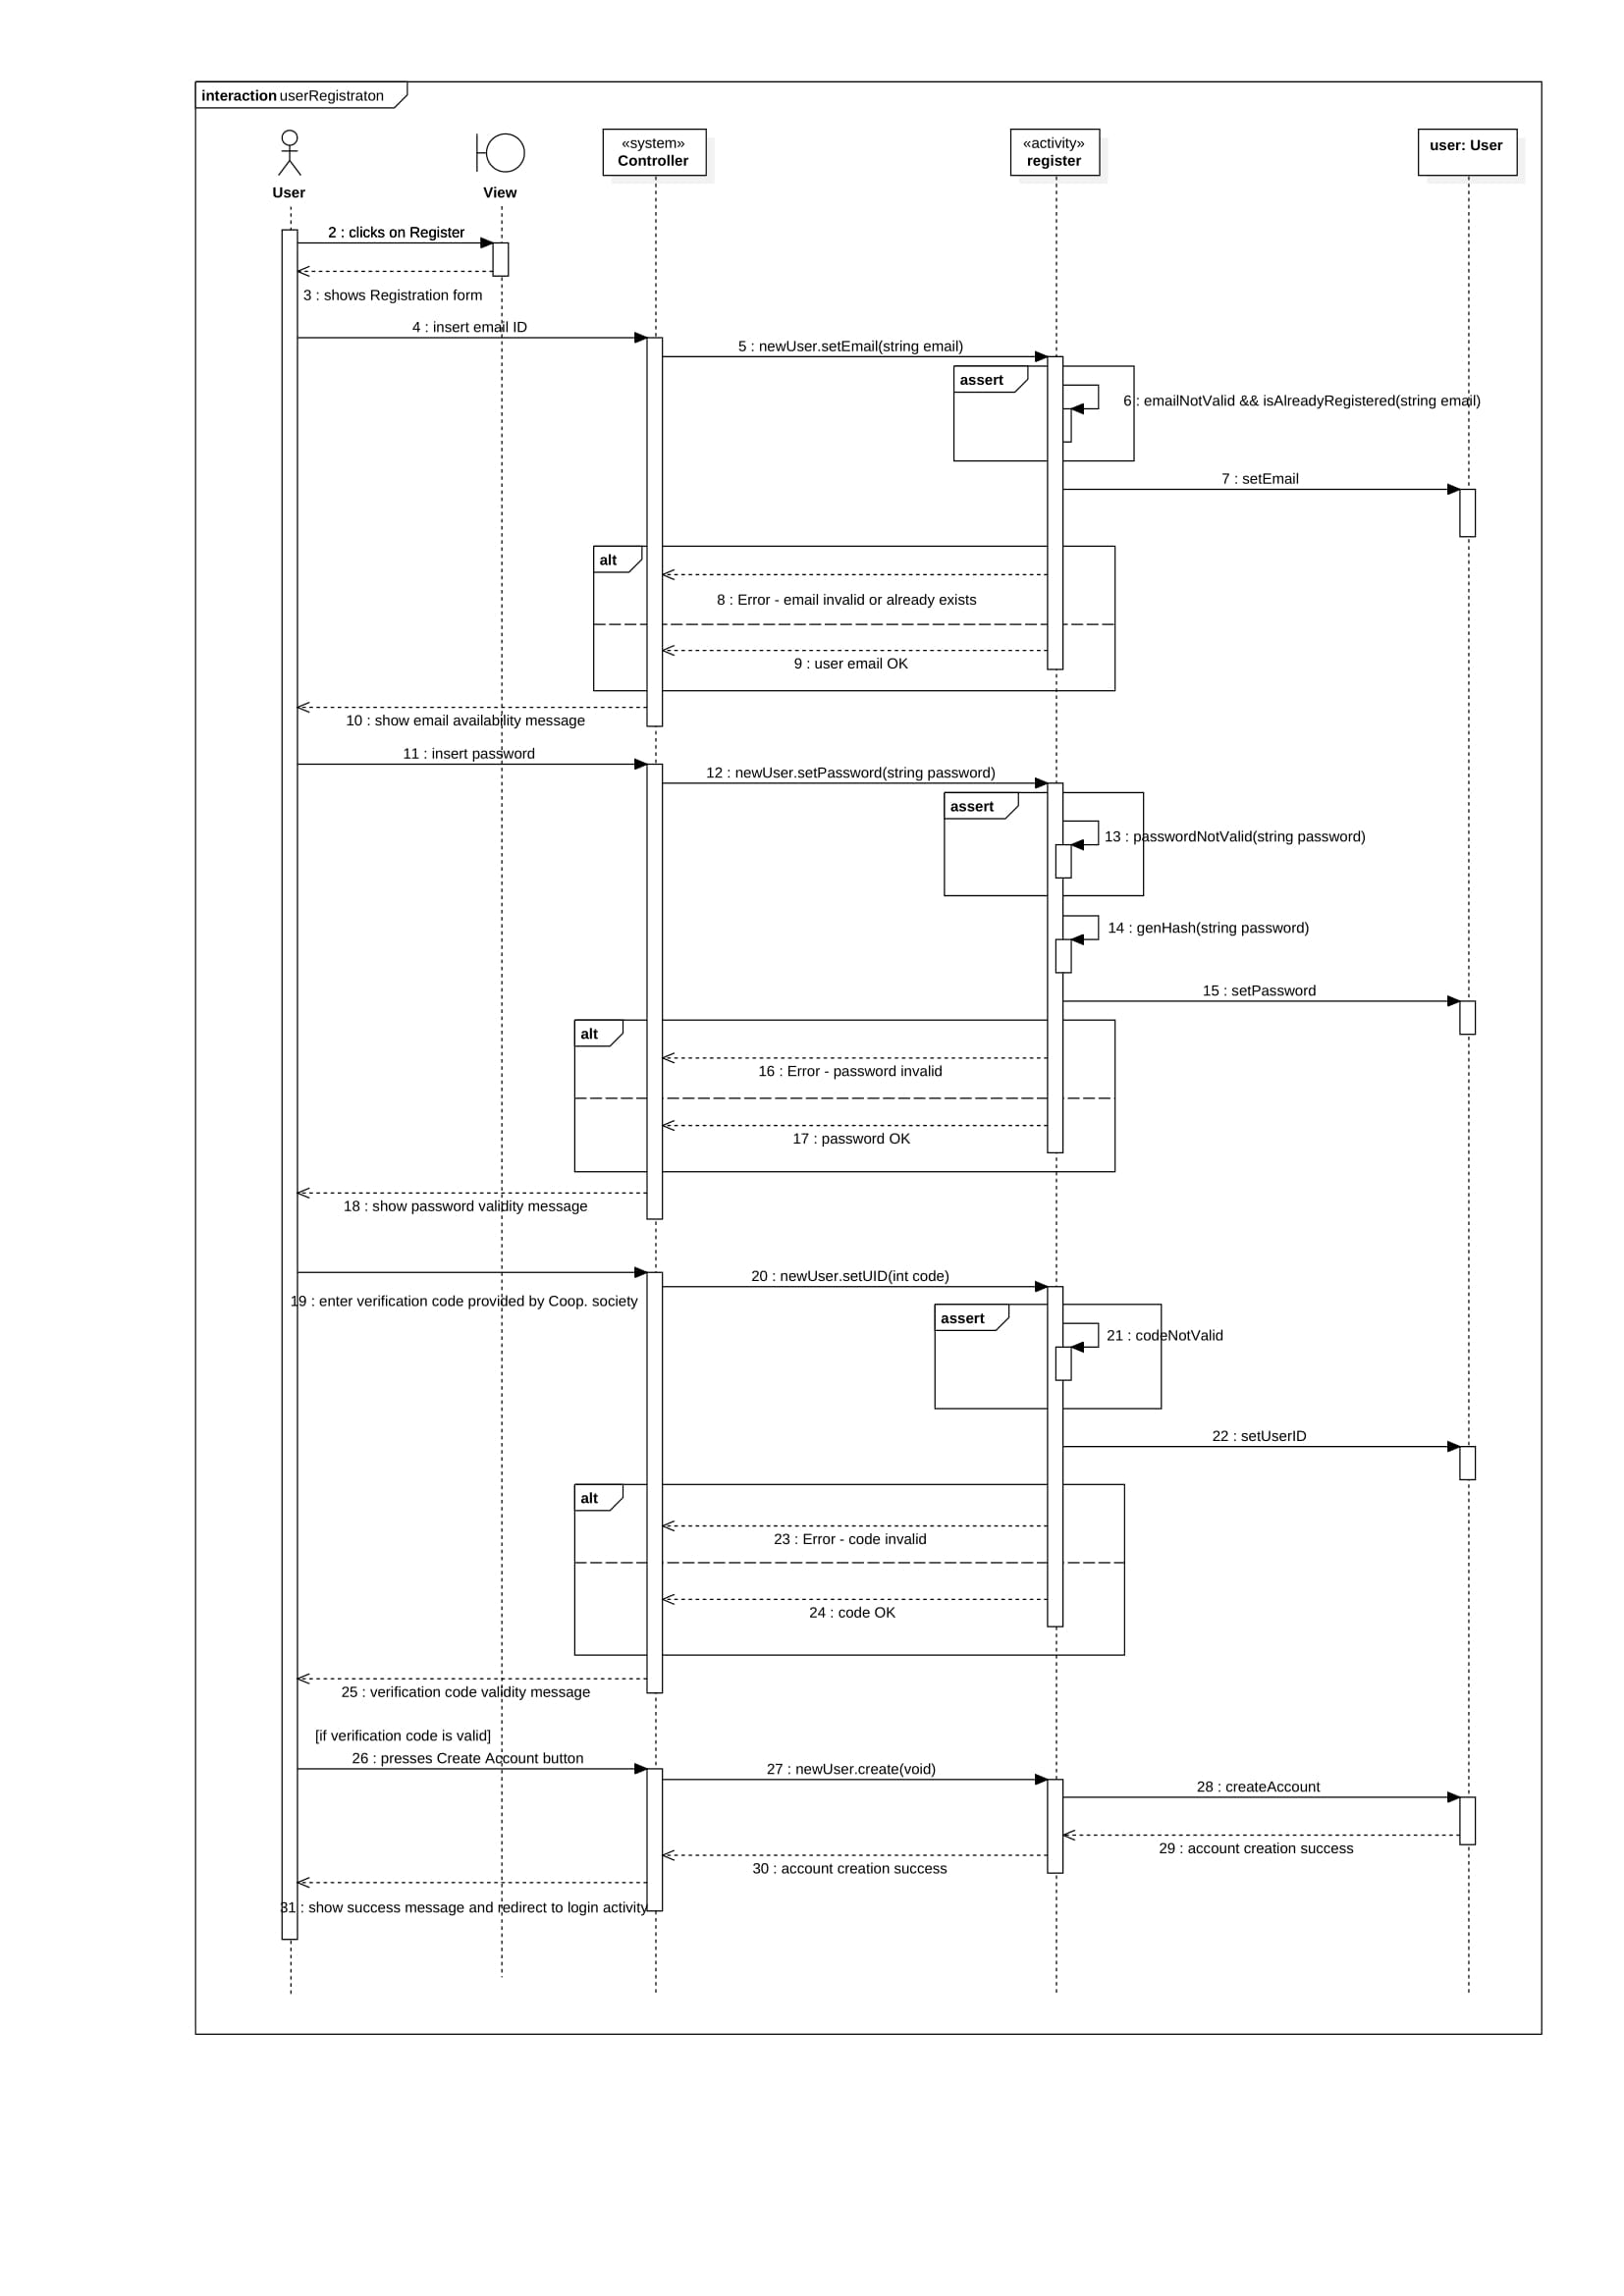
\includegraphics[scale=0.275]{user-registration-1.jpg} \\
\end{center}
% Chapter 3

\chapter{\uppercase{Implementation of the Project}} % Main chaptble to logier title
\label{ch:chap3} % For referencing
On launching the application, the user will be able to register by providing their details and user token provided by their distributor. With this, the user will be able to login and specify their requirements. They can update this regularly. The user will be prompted to enter their address and with the help of  google maps API, he/she will be able to point to their accurate location. 







%\section{\uppercase{View of Tables}}
%Sample view  is shown in Table \ref{tab:first} and an example is given in Table~\ref{tab:second}.


\section{\uppercase{Application Screenshots}}
%Examples of pictures are shown in Figure \ref{fig:one} and Figure \ref{fig:two}.
\begin{figure}[h]
\begin{center}
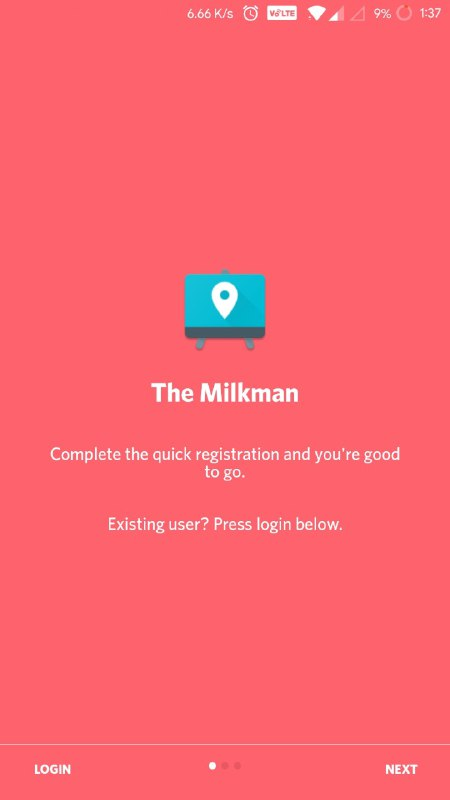
\includegraphics[scale=0.6]{3/one.jpeg}
\caption{Home page}
\label{fig:one}
\end{center}
\end{figure}

\begin{figure}[h]
\begin{center}
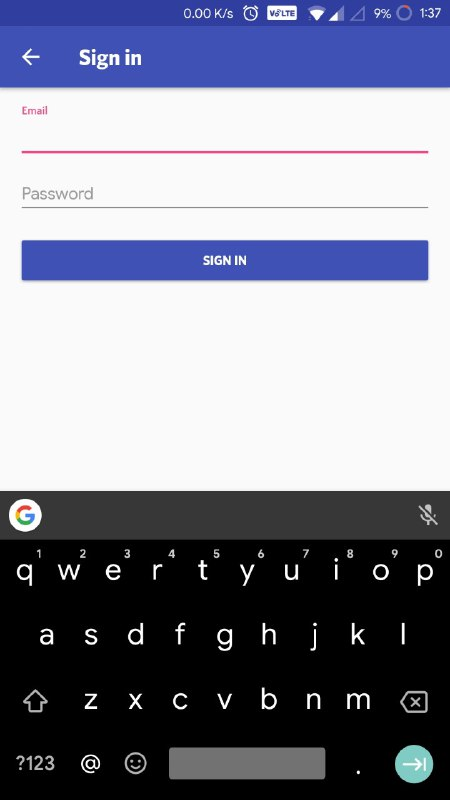
\includegraphics[scale=0.6]{3/two.jpeg}
\caption{Sign in!}
\label{fig:two}
\end{center}
\end{figure}

\begin{figure}[h]
  \begin{center}
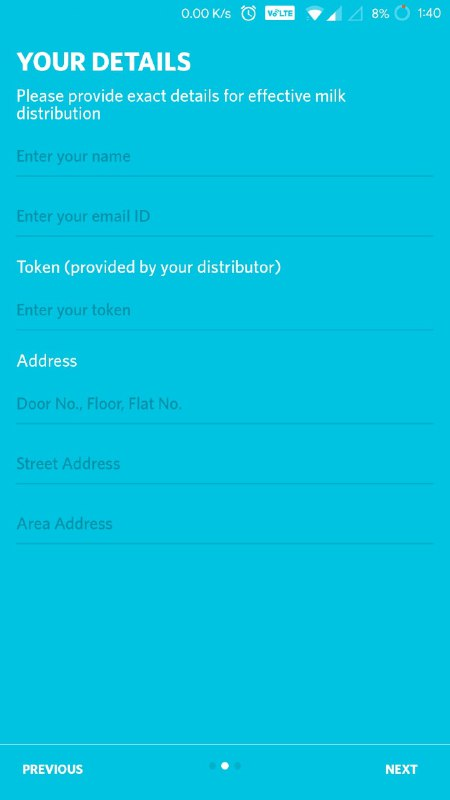
\includegraphics[scale=0.6]{3/three.jpeg}
\caption{Registration}
\label{fig:two}
\end{center}
\end{figure}

\begin{figure}[h]
  \begin{center}
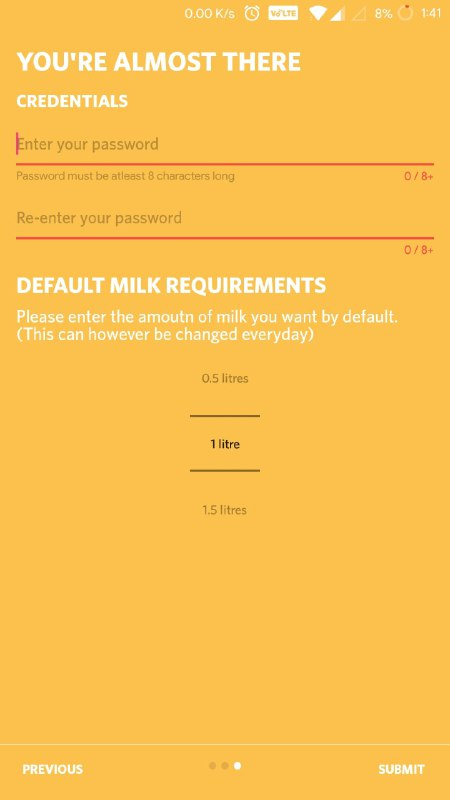
\includegraphics[scale=0.6]{3/four.jpeg}
\caption{Login and requirements}
\label{fig:two}
\end{center}
\end{figure}

\begin{figure}[h]
  \begin{center}
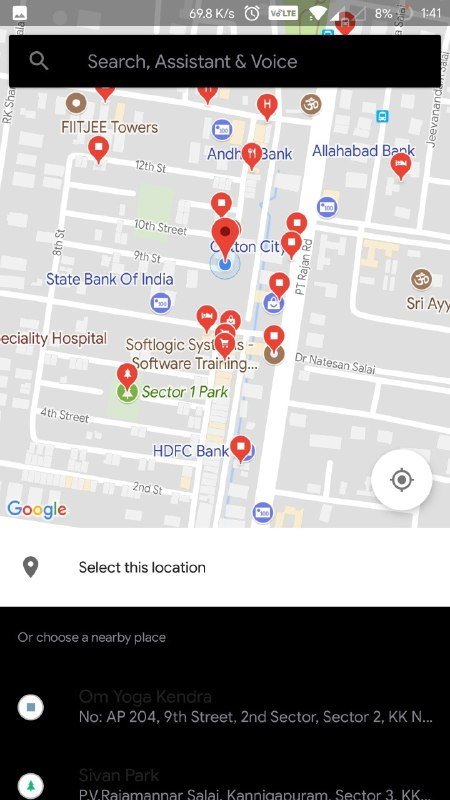
\includegraphics[scale=0.6]{3/five.jpeg}
\caption{Users latitue and longitude}
\label{fig:two}
\end{center}
\end{figure}

\begin{figure}[h]
  \begin{center}
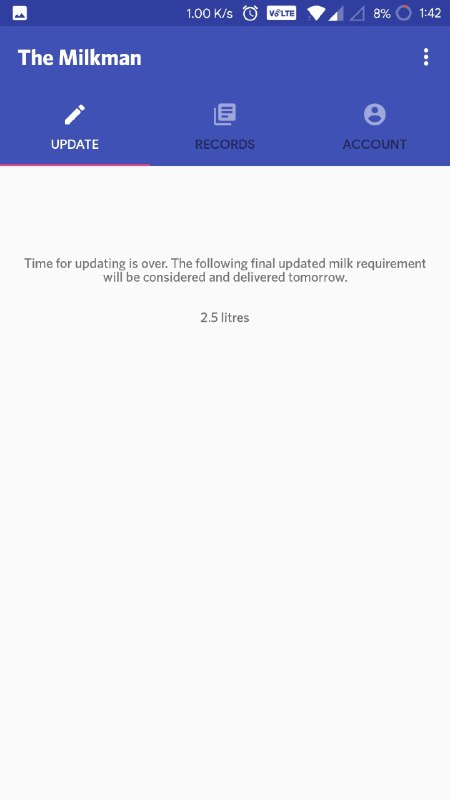
\includegraphics[scale=0.6]{3/six.jpeg}
\caption{Dashboard}
\label{fig:two}
\end{center}
\end{figure}

\begin{figure}[h]
  \begin{center}
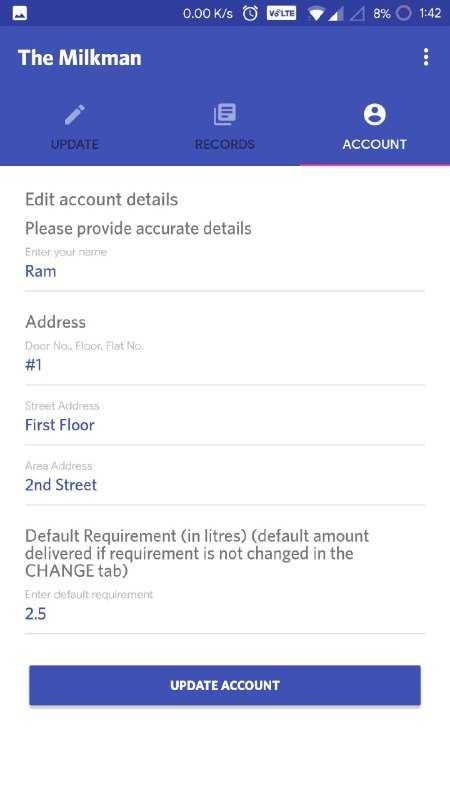
\includegraphics[scale=0.6]{3/seven.jpeg}
\caption{User details}
\label{fig:two}
\end{center}
\end{figure}

\begin{figure}[h]
  \begin{center}
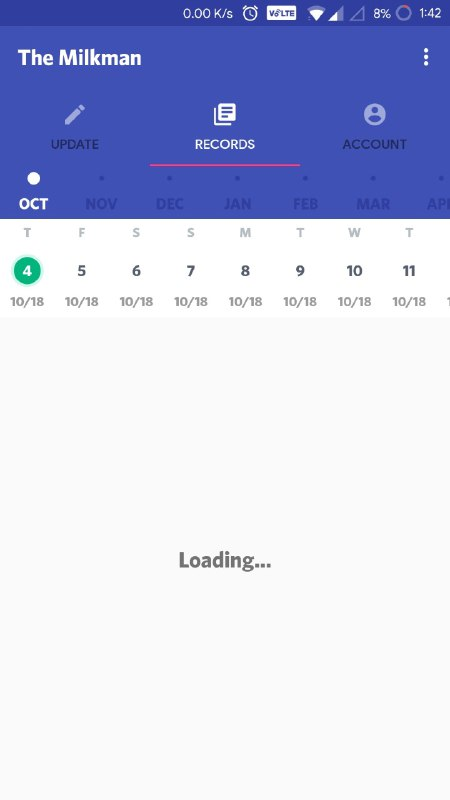
\includegraphics[scale=0.6]{3/eight.jpeg}
\caption{Consumption History}
\label{fig:two}
\end{center}
\end{figure}

\begin{figure}[h]
  \begin{center}
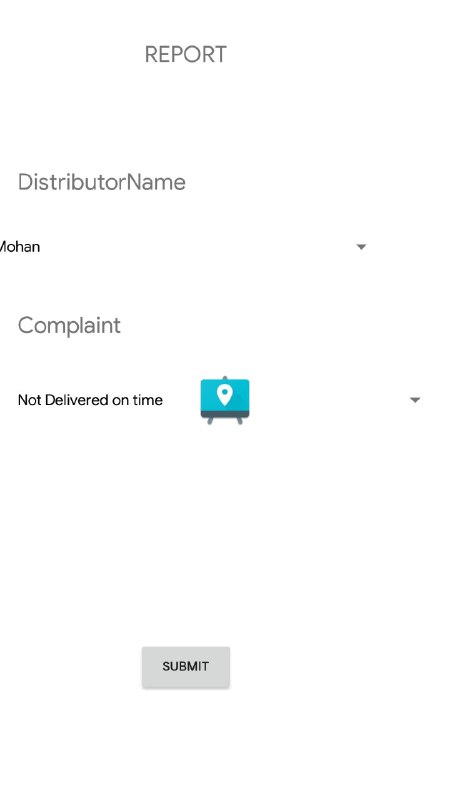
\includegraphics[scale=0.6]{3/nine.jpeg}
\caption{Complaints}
\label{fig:two}
\end{center}
\end{figure}

\begin{figure}[h]
  \begin{center}
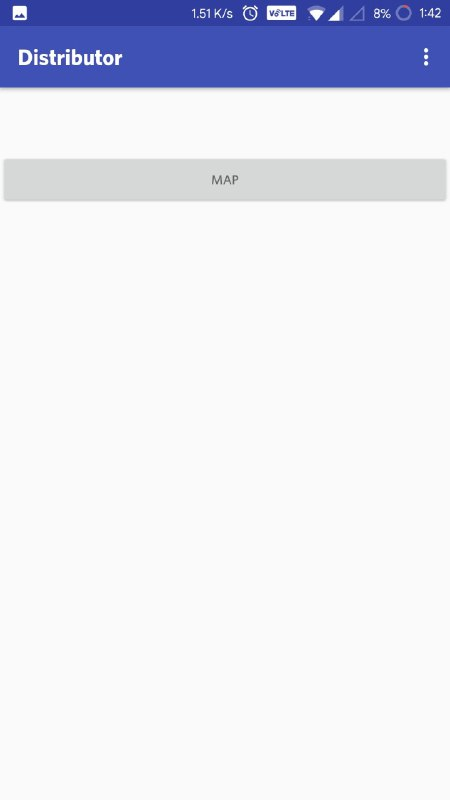
\includegraphics[scale=0.6]{3/ten.jpeg}
\caption{Distributor's interface}
\label{fig:two}
\end{center}
\end{figure}

\begin{figure}[h]
  \begin{center}
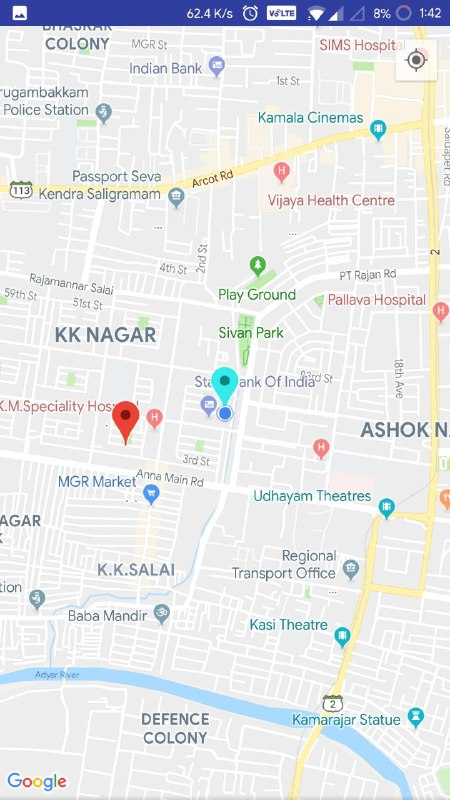
\includegraphics[scale=0.6]{3/eleven.jpeg}
\caption{Delivery}
\label{fig:two}
\end{center}
\end{figure}

\begin{figure}[h]
  \begin{center}
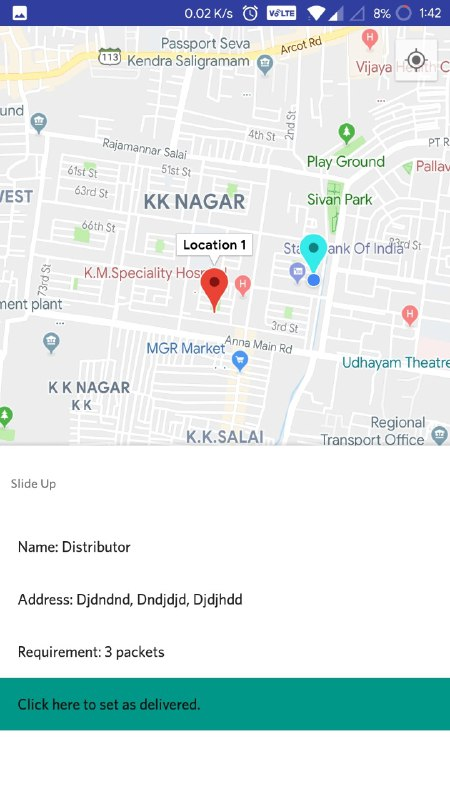
\includegraphics[scale=0.6]{3/twelve.jpeg}
\caption{Delivery }
\label{fig:two}
\end{center}
\end{figure}

\begin{figure}[h]
  \begin{center}
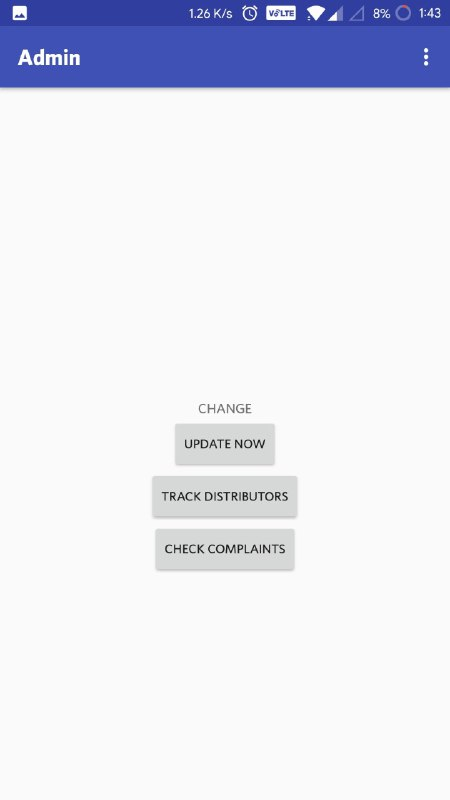
\includegraphics[scale=0.6]{3/thirteen.jpeg}
\caption{Admin Interface}
\label{fig:two}
\end{center}
\end{figure}

\begin{figure}[h]
  \begin{center}
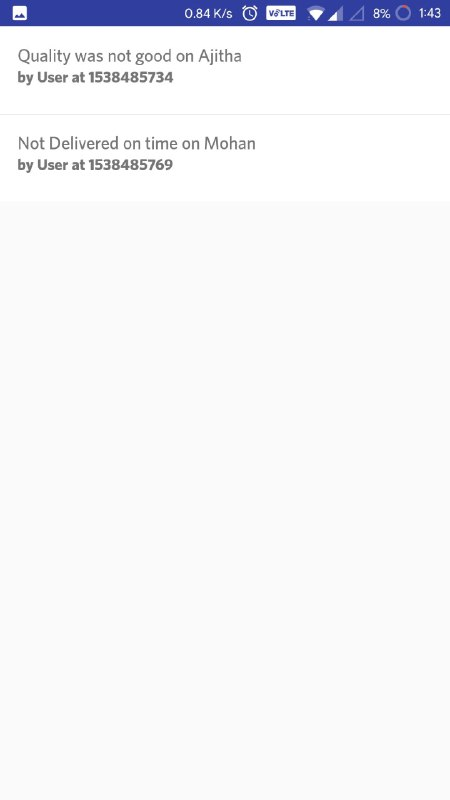
\includegraphics[scale=0.6]{3/fourteen.jpeg}
\caption{Displaying Complaints}
\label{fig:two}
\end{center}
\end{figure}








%% Chapter 4

\chapter{\uppercase{Implementation of your work}} % Main chapter title
\label{chap4} % For referencing
The implementation details of your work should be mentioned in this chapter.
\section{\uppercase{Algorithm 1}}
\begin{algorithm}
\begin{algorithmic}[1]
\State Get the number of variables $num$ 
\State Start with an empty list $x$ $[~]$
\For {each $n$ of $num$}
	\State Get the $x$
	\State  Get the $t$
	\State Get the $w$
\EndFor 
\If {$xl$ == $s$} 
	\State terminate with the failure message \textbf{failed}
\Else
	\State $z = x$
\EndIf 

\end{algorithmic}
\end{algorithm}




%% Chapter 5

\chapter{\uppercase{Results and Performance Analysis}} % Main chapter title
\label{chap5} % For referencing
This chapter should provide the details of results and the analysis of your work. Depending on the type of project, there may not be analysis. In such cases, mention the title as ``Results'' or ``Testing and Results''.


%% Chapter 6

\chapter{\uppercase{Comparison}} % Main chapter title
\label{chap6} % For referencing
This chapter is optional. Depending on the work, comparison can also be included in previous chapter.


\chapter{\uppercase{Conclusion and Future Work}}
\label{chap:conclusion}
With the massive advancements in technology, every sector has gained better improvements. Milk, being one of the basic necessities, this sector has to improve too! 
Through our application, customers and co-operative society will be able to beinfit and get their requirements in ease. 
\cleardoublepage
\phantomsection 
%\appendix
\addcontentsline{toc}{chapter}{APPENDIX}
\chapter{\uppercase{Topic 1}}
\section{\uppercase{Section 1}}
\section{\uppercase{Section 2}}
\chapter{\uppercase{Topic 2}}
\section{\uppercase{Section 1}}
\section{\uppercase{Section 2}}






%\bibliographystyle{auapalike}
\bibliographystyle{unsrt}
\nocite{*}%This gives a list of all references that includes without citation. Remove this, once the reference is cited
\phantomsection
\addcontentsline{toc}{chapter}{REFERENCES}
\begin{spacing}{1}
\bibliography{publication}
\end{spacing}

\newpage
\clearpage




\addtocontents{toc}{\protect\newpage}
\addtocontents{lot}{\protect\newpage}
\addtocontents{lof}{\protect\newpage}

\end{document}
